An \glsdesc{acr:oqe} \gls{seismicsourceinputmodel} contains a list of sources
belonging to a finite set of possible typologies. Each source type is defined
by a set of parameters - called source data - which are used to specify the
source geometry and the properties of seismicity occurrence.

Currently the \glsdesc{acr:oqe} supports the following source types:

\begin{itemize}

    \item Sources for modelling distributed seismicity:

    \begin{itemize}

        \item \Gls{pointsource} - The elemental source type used to model
        distributed seismicity. Grid and area sources (described below) are
        different containers of point sources.

        \item \Gls{areasource} - So far, the most frequently adopted source
        type in national and regional PSHA models.

        \item \Gls{gridsource} - A replacement for area sources admitting
        spatially variable seismicity occurrence properties.

    \end{itemize}

    \item Fault sources with floating ruptures:

    \begin{itemize}

        \item \Gls{simplefaultsource} - The simplest fault model in the
        \glsdesc{acr:oqe}. This source is habitually used to describe shallow
        seismogenic faults.

        \item \Gls{complexfaultsource} - Often used to model subduction
        interface sources with a complex geometry.

    \end{itemize}

    \item Fault sources with ruptures always covering the entire fault
    \surface:

    \begin{itemize}

        \item \Gls{charfaultsource} - A typology of source where ruptures
        always fill the entire fault surface.

    \end{itemize}

\end{itemize}

The \glsdesc{acr:oqe} contains some basic assumptions for the definition of
these source typologies:

\begin{itemize}

    \item In the case of area and fault sources, the seismicity is
    homogeneously distributed over the source;

    \item Seismicity temporal occurrence follows a Poissonian model.

\end{itemize}



\subsection{Source typologies for modelling distributed seismicity}
\input{oqum/hazard/00a_sources_distributed_seismicity}

\subsection{Fault sources with floating ruptures}
\input{oqum/hazard/00a_sources_floating_ruptures}

\subsection{Fault sources without floating ruptures}
\subsubsection{Characteristic faults}
\label{desc_characteristic_fault}
\index{Source type!fault!characteristic}
\index{Characteristic fault|see{Source type}}

The characteristic fault source is a particular typology of fault created
with the assumption that its ruptures will always cover the entire fault
surface. As such, no floating is necessary on the surface. The characteristic fault may still take as input a magnitude frequency distribution. In this case, the fault surface can be represented either as a \gls{simplefaultsource} surface or as a \gls{complexfaultsource} surface or as a combination of rectangular ruptures as represented in
Figure~\ref{fig:char_fault_source}. Mutiple surfaces containing mixed geometry types are also supported. 


\begin{figure}[htb]
\centering
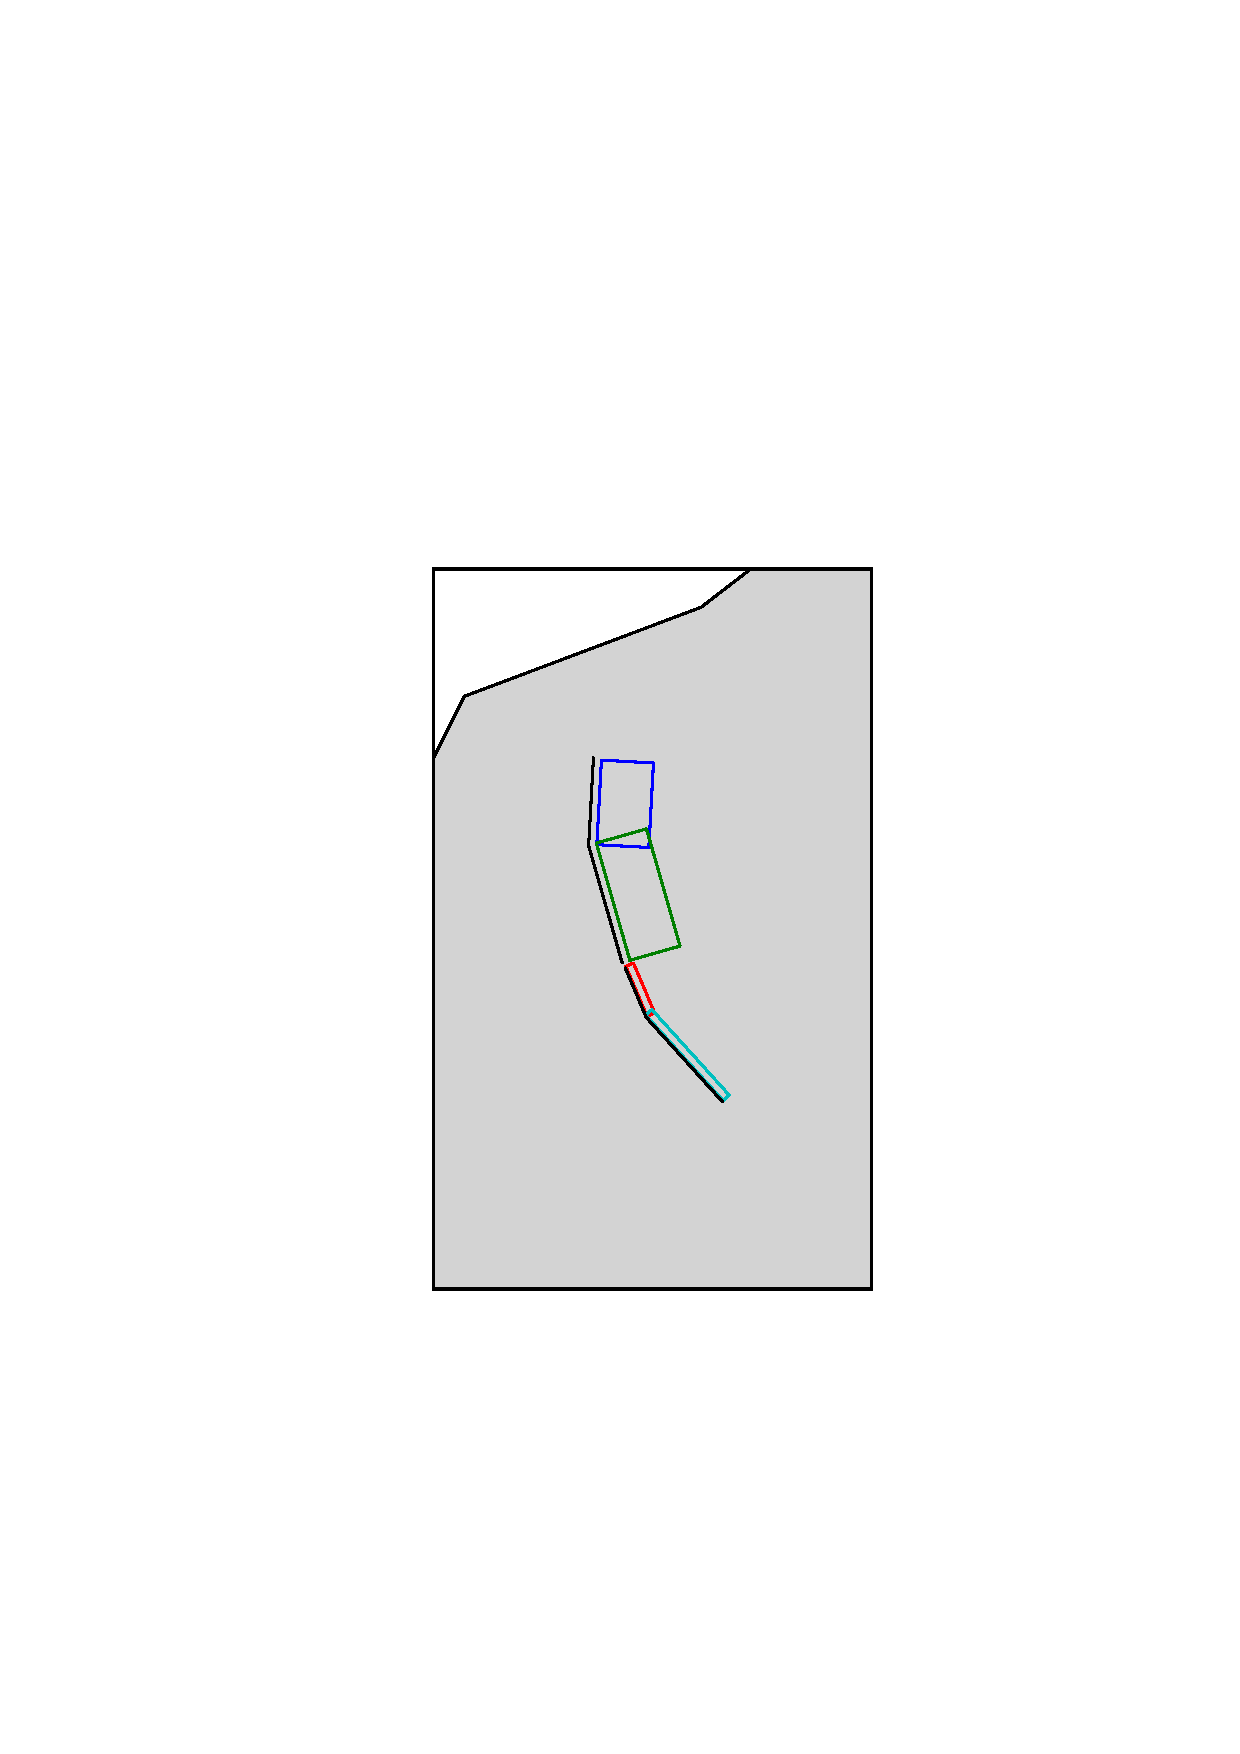
\includegraphics[trim=5cm 7cm 5cm 7cm, clip, width=10cm]{figures/hazard/multi_surface.pdf}
\caption{Geometry of a multi-segmented characteristic fault composed of four
         rectangular ruptures as modelled in OpenQuake.}
\label{fig:char_fault_source}
\end{figure}

\paragraph{Source data}

\begin{itemize}

    \item The characteristic rupture surface is defined through one of the
    following options:

        \begin{itemize}

            \item A list of rectangular ruptures (``planar surfaces'')

            \item A \gls{simplefaultsource} geometry

            \item A \gls{complexfaultsource} geometry

        \end{itemize}

    \item A \gls{frequencymagnitudedistribution}.

    \item Rake angle (specified following the Aki-Richards convention; see
          \citet{aki2002}).

    \item Upper and lower depth values limiting the seismogenic interval.

\end{itemize}
A comprehensive example enumerating the possible rupture surface configurations is shown below. 

\input{oqum/hazard/verbatim/input_characteristic_fault}

\subsubsection{Non-Parametric Fault}
\label{desc_nonparametric_fault}
\index{Source type!fault!nonparametric}
\index{Non-Parametric fault|see{Source type}}

The non-parametric fault typology requires that the user indicates the rupture properties (rupture surface, magnitude, rake and hypocentre) and the corresponding probabilities of the rupture. The probabilities are given as a list of floating point values that correspond to the probabilities of $0, 1, 2, \ldots ... N$ occurrences of the rupture within the specified investigation time. Note that there is not, at present, any internal check to ensure that the investigation time to which the probabilities refer corresponds to that specified in the configuration file. As the surface of the rupture is set explicitly, no rupture floating occurs, and, as in the case of the characteristic fault source, the rupture surface can be defined as either a single planar rupture, a list of planar ruptures, a \gls{simplefaultsource} geometry, a \gls{complexfaultsource} geometry, or a combination of different geometries.

An comprehensive example enumerating the possible configurations is shown below:

\input{oqum/hazard/verbatim/input_nonparametric_source}


